\begin{figure}[t]
  \centering
  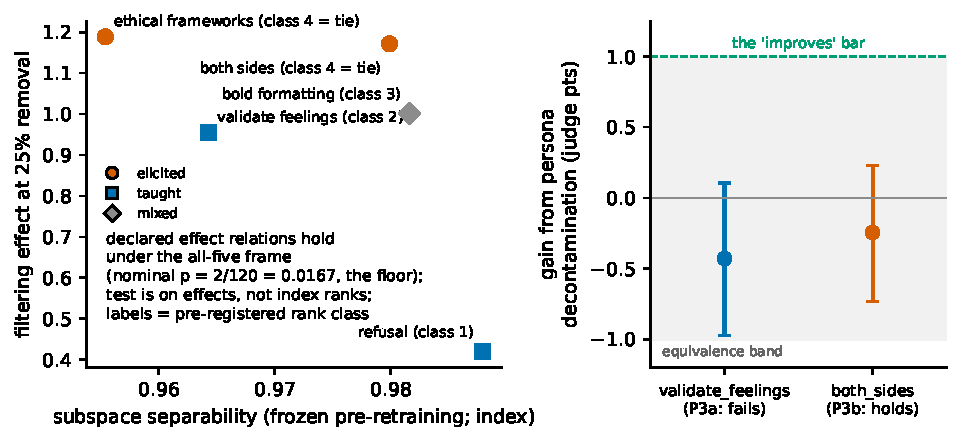
\includegraphics[width=\linewidth]{FIG-0_headline.pdf}
  \caption{Post-result editorial composite of the canonical H2 ordering
    plot (left) and H3 causal plot (right). The pre-fixed headline rule
    selected FIG-7 when H3 ran; this composite adds FIG-6 context, while
    both single-panel figures remain canonical. Left: the five filtering
    effects at 25\% removal satisfy all nine declared cross-class relations
    (refusal most filterable). Under the declared all-five permutation frame,
    the nominal exact rank-tail is $p = 2/120 = 0.0167$. This is not a
    noise-aware or fully fresh five-effect p-value: two effects were already
    known when the final set was fixed, and each target retrain is single-seed.
    Point labels show the pre-registered rank classes, with \behavior{both\_sides} and
    \behavior{ethical\_frameworks} tied in class 4; no within-class order
    was predicted. The measured separability index mis-ranks
    \behavior{validate\_feelings} in-sample, so this order test is on
    filtering effects, not a claim that the index perfectly rank-orders
    outcomes. Right: persona-subspace decontamination fails P3a for
    \behavior{validate\_feelings} (improvement $-0.430$, CI
    [$-0.975$, $+0.105$], below the $+1.0$ bar) while P3b holds for
    \behavior{both\_sides} (improvement $-0.245$, inside the $|d|<1.0$
    equivalence band). The declared ordering relations held, but this
    frozen post-training decontamination test did not support the
    persona-bundling mechanism. (data:
    \texttt{results/h1h2/h1\_h2\_measurements.json},
    \texttt{results/h3/h3\_analysis.json}; regenerate:
    \texttt{scripts/22\_figures.py})}
  \label{fig:headline}
\end{figure}
